\documentclass[12,a4paper]{article}
\usepackage{classiccomputing}

\newcommand\postertype{lightgray}

\begin{document}

\makecclogo

\author{} % owner of the device, also used as "Author" in PDF export
\title{Auerswald COMmander Basic.2}
\def\subtitle{ISDN-Telefonanlage}
\def\introduction{Markteinführung 2006}
\makeheader{35}{40} % title size 35, subtitle size 40

\includeimage {images/Auerswald_COMB2_mainboard1.png}{0.5}

\makebullets{
    Land: Deutschland \newline
    19" 3HE-BGT oder Wandgehäuse \newline
   
    Modulare Bauweise, Einsteckkarten: \newline
    8x ISDN-S0 (Basisanschluss) \newline
    1x ISDN-S2m (E1 / Primärmultiplex) \newline
    8x a/b (analog / POTS) \newline

    Leistungsaufnahme: $\sim$10W \newline
}

\makemain{
    Moderne Telefonanlage mit Linux \newline
    Per Webinterface konfigurierbar \newline \newline
    Gute Unterstützung von analogen Fax/Modem-Verbindungen (volle 56k erreichbar) \newline
}

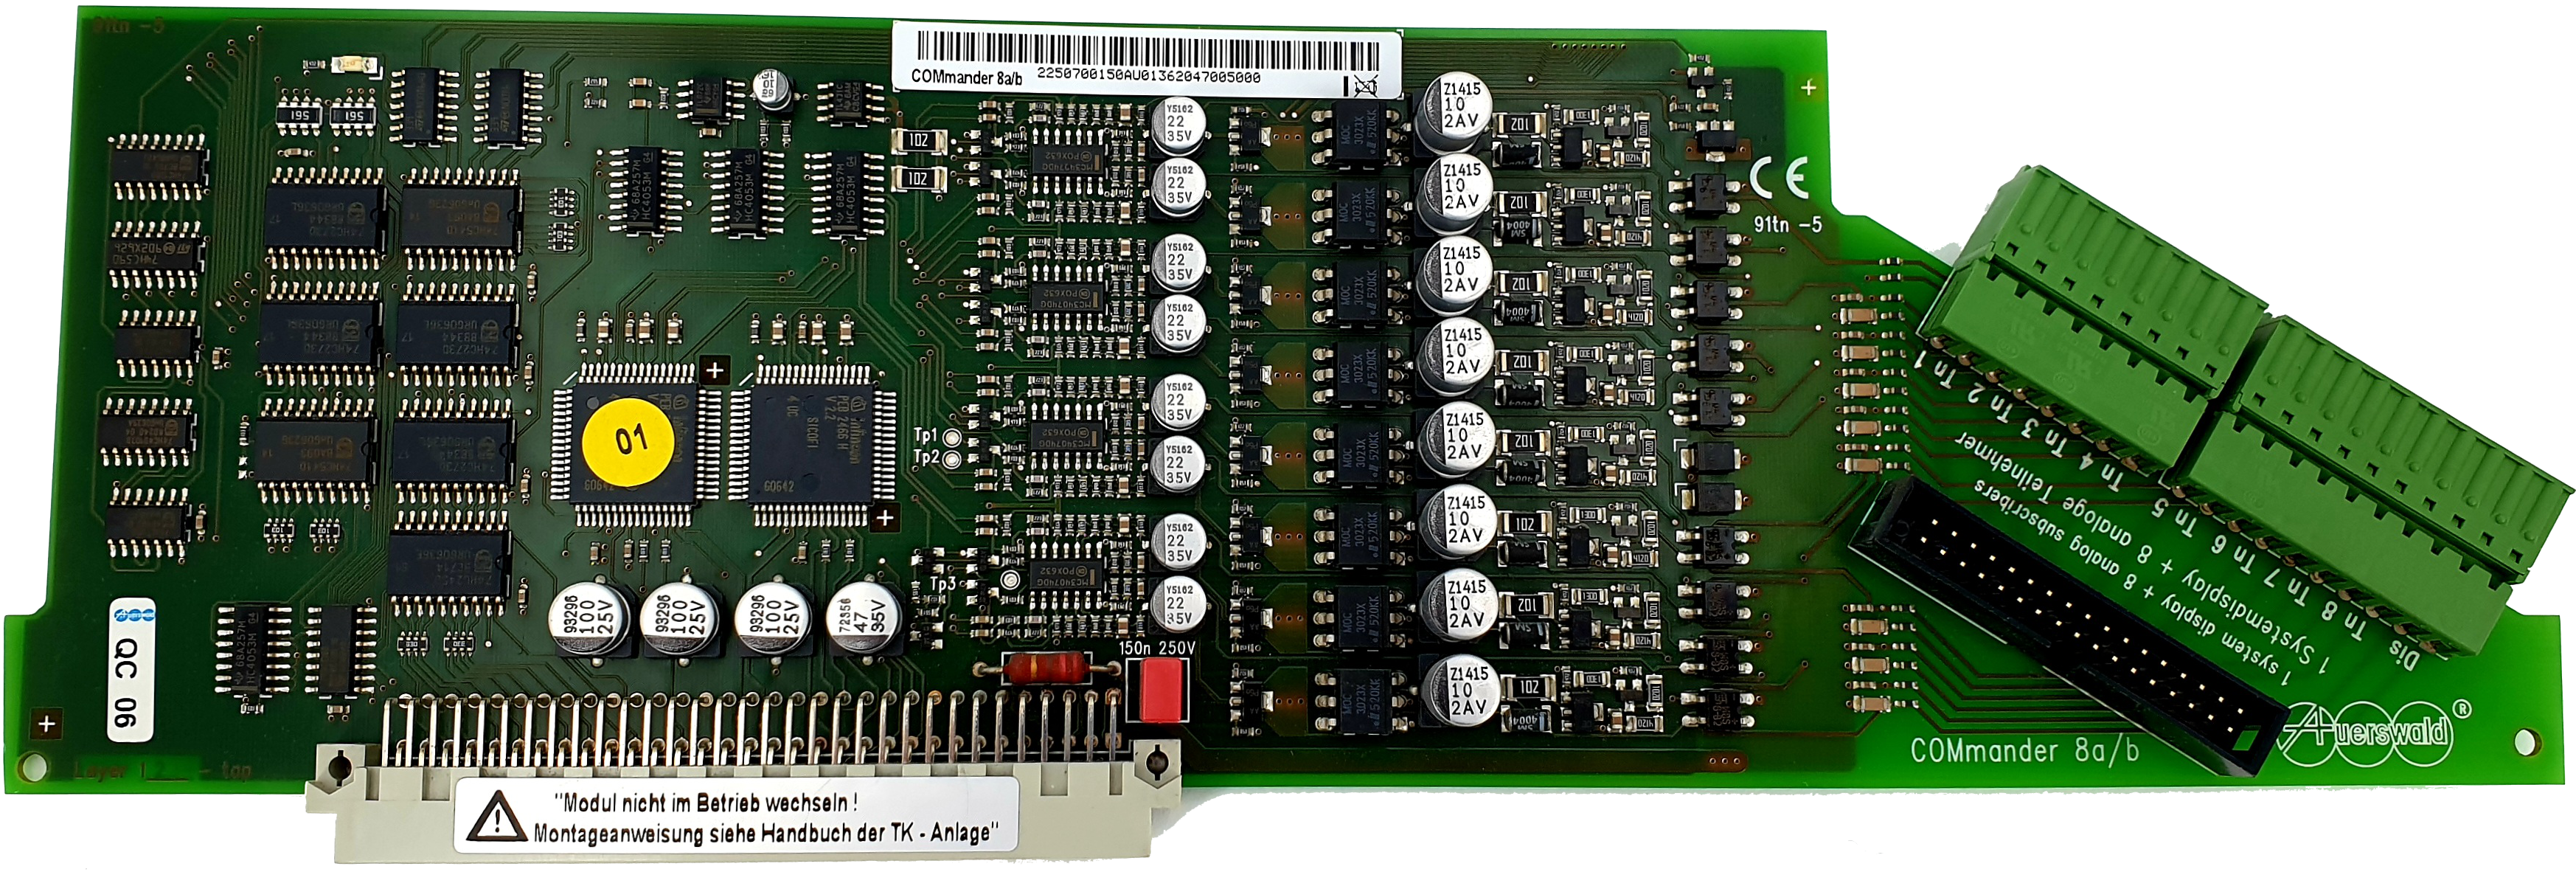
\includegraphics[width=0.8\linewidth]{images/Auerswald_COMmander_8ab_top.png}

\makefooter

\end{document}